\documentclass{article}
\usepackage{graphicx} % Required for inserting images
\graphicspath{ {./images/} }
\usepackage{enumitem}
\usepackage[utf8]{inputenc}
\usepackage{bm}
\usepackage{amsmath}
\usepackage{mathtools}% Loads amsmath
\usepackage{amssymb}
\usepackage{multicol}
\usepackage{xcolor}

\usepackage{arydshln}

\setlength{\dashlinedash}{4pt}
\setlength{\dashlinegap}{4pt}

\allowdisplaybreaks
\usepackage{geometry}
 \geometry{
 a4paper,
 total={170mm,257mm},
 left=17mm,
 top=20mm,
 }
% Footer
\usepackage{fancyhdr}

\pagestyle{fancy}
\fancyhf{} 
\fancyfoot[L]{MATH3202 A1}
\fancyfoot[C]{Hugo Burton, Lucy Ochre, and Anna Henderson}
\fancyfoot[R]{\thepage}
\renewcommand{\headrulewidth}{0pt} % Remove the line at the top of the page
\renewcommand{\footrulewidth}{0.4pt} % Add a line just above the footer

% cmds
\renewcommand*{\thesection}{\Alph{section}}

\begin{document}

\begin{titlepage}
    \begin{center}
        \vspace*{1cm}
            
        \Huge
        \textbf{MATH3202 Linear Programming}
            
        \vspace{0.5cm}
        \Large
        Assignment 1
            
        \vspace{1.5cm}
            
        \textbf{Hugo Burton} (s4698512);\\ \textbf{Lucy Ochre} (s4699043); \&\\ \textbf{Anna Henderson} (s4641893)\\
        \bigskip
        \text{March 2023}
        \vfill
        \text{(Using Anna's Data)}
        \vfill
        
        %\includegraphics[width=0.4\textwidth]
        \centering{
            
\includegraphics[width=0.25\textwidth]{MSS-logo2}\\
        }
        \vspace{2cm}
        \Large
        UQ Mathematics\\
        The University of Queensland\\
        Australia\\
        Course code: MATH3202
    \end{center}
\end{titlepage}

\section{Report to Boss}
%A general mathematical formulation of the problem, including definitions of sets, data, variables, objective function and constraints. 7 marks • A Python file with the problem modelled for Gurobi. This should be easy to relate back to the formulation. Your boss will attempt to execute this model. 5 marks

\bigskip

\subsection{Sets}
\bigskip
In a linear programming problem, sets are a collection of defined objects required to model the problem. They have been described in the following table:\\
\bigskip
\renewcommand\baselinestretch{1.5}
\begin{table}[h]
    \centering
    \color{black}
    \begin{tabular}{|c:l|}
        \hline
        \textbf{Set} & \textbf{Description} \\
        \hline
        \(N\) & Nodes \\ \hdashline
        \(S\) & Suppliers - a subset of Nodes \((S\subset N)\)\\ \hdashline
        \(P\) & Pipelines\\ \hdashline
        \(T\) & Days\\
        \hline
    \end{tabular}
    \caption{Table of sets within the model}
    \label{tab:sets}
\end{table}
\renewcommand\baselinestretch{1}\\
The set N of nodes are the set of points on the grid where either gas is demanded, or gas is produced. The set of nodes includes the gas supplier plants.\\
\\
The set S of suppliers is a subset of the set of nodes that contains only the nodes at which gas is produced.\\
\\
The set P of pipelines is the edges of the graph which connect nodes to one another. The pipes are defined as an id and which two nodes they connect. Gas can flow either direction in any given pipe.\\
\\
The set T of days is trivial but is a set of the day numbers in a two-week period - indexed from 0 to 13 inclusive.


\bigskip
\subsection{Data}
\bigskip
The data for this linear programming problem has been summarised in the following table. This is the information that gets used later on within the objective function and the constraints. The units for each piece of data has also been listed. \\
\\
Some values in the data are constants, but can still be considered data as these may change from one gas network to another gas network.
\bigskip
\renewcommand\baselinestretch{1.5}
\begin{table}[h]
    \centering
    \color{black}
        \begin{tabular}{|c:l:c|}
        %\begin{tabular*}{375pt}{@{\extracolsep{\fill}}|c l c|}
        \hline
        \textbf{Variable} & \textbf{Description} & \textbf{Units} \\
        \hline
        \(d_{n,t}\) & Demand of gas at node \(n\in N\) on day \(t \in T\) & MJ \\ \hdashline
        \(a_n\) & Capacity of each node (normal nodes have 0 cap) & MJ \\ \hdashline
        \(c_n\) & Cost of gas at node n & \(\$\) \\ \hdashline
        \(l_p\) & Length of pipeline \(p\in P\) & km \\ \hdashline
        \((f_p, \tau_p)\) & (Node \(n\in N\) pipe \(p \in P\) is from, Node \(n \in N\) pipe \(p \in P\) goes to) & \(\cdot\) \\ \hdashline
        \(M\) & Maximum flow of gas through any pipe per day & \(\frac{MJ}{\text{day}}\) \\ \hdashline
        \(G\) & Maximum gas per supplier over 2 weeks & MJ \\ \hdashline
        \(\lambda\) & Cost of moving gas through pipe per MJ per km & \(\frac{\$}{MJ\hspace{0.1cm} km}\) \\ \hdashline
        \(\epsilon\) & Daily cost of storing imbalance of gas in pipe per MJ & \(\frac{\$}{MJ}\) \\
        \hline
    \end{tabular}
    \caption{Table outlining the data present within the model}
    \label{tab:data}
\end{table}
\renewcommand\baselinestretch{1}
\bigskip
\newpage
\subsection{Variables}
\bigskip
The decision variables have been described in the following table (3). These are the unknown quantities that are to be determined in the problem's solution. As this is a linear programming problem, these variables take values in the reals.
\renewcommand\baselinestretch{1.5}
\begin{table}[h]
    \centering
    \color{black}
    \begin{tabular}{|c:l|}
        \hline
        \textbf{Variable} & \textbf{Description} \\
        \hline
        \(x_{n,t}\) & Gas produced at node \(n\in N\) on day \(t \in T\) \\ \hdashline
        \(y_{p,t}\) & Gas that has flowed into pipe \(p\in P\) on day \(t \in T\) \\ \hdashline
        \(z_{p,t}\) & Gas that has flowed out of pipe \(p\in P\) on day \(t \in T\) \\ \hdashline
        \(\delta_{p,t}\) & Difference in gas flowing in and out of pipe \(p\in P\) on day \(t \in T\) \\
        \hline
    \end{tabular}
    \caption{Table of decision variables}
    \label{tab:vars}
\end{table}
\renewcommand\baselinestretch{1}
\bigskip
\subsection{Objective}
\bigskip
The objective of this problem is to minimise the costs associated with producing gas as well as distributing it to where it is demanded. We can represent the objective mathematically by minimising the following expression:

\[\min{\left\{\sum_{t\in T}\left[\sum_{n\in N}(c_n x_{n,t}) + \sum_{p \in P}\left(\lambda l_p y_{p,t} + \epsilon\delta_{p,t}\right)\right]\right\}}\]
\\
Observe how this factors in the additional (logistical) cost of moving the gas through the pipeline, \(\lambda\), (per MJ of gas moved per km of pipe) as well as storing any imbalance of gas in the pipes, \(\epsilon\), (per MJ for a day).\\
\\
In this gas network, \(\lambda = \$0.01 \hspace{0.1cm}\frac{\$}{MJ \hspace{0.1cm} day}\), and \(\epsilon = \$0.1 \hspace{0.1cm}\frac{\$}{MJ}\).

\bigskip
\subsection{Constraints}
\bigskip
\subsubsection{Generator Capacity}
The gas produced at each node N must of course be less than or equal to its respective capacity. Note, we have defined all nodes \(n \in N\) as generators, even though it's only a small subset \((s \in S)\) which actually produces gas. Hence all regular nodes have a capacity of \(0\). This is represented mathematically as

\[x_{n,t}\leq a_n, \hspace{1cm} \forall n\in N \hspace{0.5cm} \forall t \in T\]
\\
We also have

\[x_{n,t} = 0, \hspace{1cm} \forall n\in N \setminus S \hspace{0.5cm} \forall t \in T\]
... as we cannot produce gas at a regular node.

\bigskip


\subsubsection{Gas Flow Constraint}

Importantly, we must constrain on the flow of gas at each node. Specifically the gas produced at the node (if any) plus the inflow of gas to the node (\(z_{p,t}\) where \(\tau_p=n\)) must equal the gas used at that node (demand) plus the outflow of gas onto other nodes (\(y_{p,t}\) where \(f_p=n\)). Mathematically this is written as

%\[x_{n,t}+\sum_{p\in P | \tau_p = n}y_{p,t} = d_n + \sum_{p\in P | f_p = n}y_{p,t}\]
\[x_{n,t}+\sum_{\substack{p\in P \\ \tau_p = n}}z_{p,t} = d_{n,t} + \sum_{\substack{p\in P \\ f_p = n}}y_{p,t}, \hspace{1cm} \forall n \in N \hspace{0.5cm} \forall t \in T\]

% Communication 2 constraint
\subsubsection{Pipeline Flow Capacity}

% The specific amount varies. See note below.
Pipelines have a maximum capacity of \(M\) MJ per day. Observe that for completeness, it is important to set bounds on both the inflow and outflow of gas.\\
\begin{align}
    y_{p,t} &\leq M \hspace{0.3cm} (MJ), \hspace{1cm} \forall p \in P \hspace{0.51cm} \forall t \in T \\
    z_{p,t} &\leq M \hspace{0.3cm} (MJ), \hspace{1cm} \forall p \in P \hspace{0.51cm} \forall t \in T
\end{align}\\
In this gas network, the maximum capacity of each pipe is \(M = 452 \hspace{0.1cm} \frac{MJ}{\text{day}}\)
% I've defined M in the data as the maximum capacity. We didn't discuss this today but it's definitely a piece of data because it varies from gas grid to gas grid (even between the three of us).

\bigskip
% Communication 4
\subsubsection{Supplier capacity}
\bigskip

The suppliers of gas have a maximum amount of gas they can produce for the entire two-week period. This is denoted as data by \(G\) and written as:

\[\sum_{t\in T} x_{n,t} \leq G, \hspace{1cm} \forall n \in N\]

\noindent
In this gas network, each of the supplier's maximum production capacity for the fortnight is \(G = 10,227\) MJ
\subsubsection{Surplus / Deficit of Gas - Effective Storage}
Pipelines can be considered as storage of gas due to their collective enormous volume. As a result, we can use gas (demand) on a different day from when the gas was produced - effectively storing a surplus or deficit of gas for each pipe on any given day.\\
\begin{align}
        \delta_{p, t} &\geq y_{p, t} - z_{p, t} \hspace{0.3cm} (MJ), \hspace{1cm} \forall p \in P \hspace{1cm} \forall t \in T \\
        \delta_{p, t} &\geq - (y_{p, t} - z_{p, t}) \hspace{0.3cm} (MJ), \hspace{1cm} \forall p \in P \hspace{1cm} \forall t \in T
\end{align}
\\
Overall, net gas produced - net gas used must equal 0 for the two-week period.\\
\[\sum_{t\in T}y_{p,t} = \sum_{t\in T}z_{p,t} \hspace{0.3cm} (MJ), \hspace{1cm} \forall p \in P\]
\\
Gurobi re-rewrites this to be in the form
\\
\[\sum_{t\in T}y_{p,t} - \sum_{t\in T}z_{p,t} = 0 \hspace{0.3cm} (MJ), \hspace{1cm} \forall p \in P\]

\subsubsection{Non-negativity}
\bigskip
Non-negativity constraints are (fortunately) given to us when using Gurobi, however, it is still important that they are defined in the mathematical model for understanding and completeness.\\
\\
We have

\[x_{n,t} \geq 0, \hspace{1cm} \forall n \in N \hspace{0.5cm} \forall t \in T\]
... as gas-producing nodes (gas stations) produce a non-negative amount of gas.
We also have

\[y_{p,t} \geq 0, \hspace{1cm} \forall p \in P \hspace{0.5cm} \forall t \in T\]
\[z_{p,t} \geq 0, \hspace{1cm} \forall p \in P \hspace{0.5cm} \forall t \in T\]
Also, observe that
\[\delta_{p,t} \geq 0, \hspace{1cm} \forall p \in P \hspace{0.5cm} \forall t \in T\]
however, this is made redundant by the constraints in equations (3) and (4).
\bigskip


\bigskip
\subsection{Solution}
\bigskip

After running this problem through Gurbobi, it was found that the optimal total cost (without any limit on imbalance) was \(\$2,460,286.7\) to produce and move the gas around the network. This equated to producing 32,706 MJ of gas over the two-week period. The table below summarises the production of gas from each supplier node over this period.\\
\\
\renewcommand\baselinestretch{1.5}
\begin{table}[h]
    \centering
    \color{black}
    \begin{tabular}{|c:c:c:c:c|}
        \hline
        \textbf{Day} & \textbf{Supplier Node 2} & \textbf{Supplier Node 35} & \textbf{Supplier Node 35} & \textbf{Supplier Node 41} \\
        \hline
        Day 1 & 462 & 894 & 564 & 704 \\ \hdashline
        Day 2 & 462 & 955 & 514 & 704 \\ \hdashline
        Day 3 & 462 & 955 & 503 & 704 \\ \hdashline
        Day 4 & 462 & 952 & 484 & 704 \\ \hdashline
        Day 5 & 462 & 912 & 502 & 704 \\ \hdashline
        Day 6 & 462 & 340 & 268 & 704 \\ \hdashline
        Day 7 & 462 & 193 & 175 & 704 \\ \hdashline
        Day 8 & 462 & 941 & 515 & 704 \\ \hdashline
        Day 9 & 462 & 899 & 542 & 704 \\ \hdashline
        Day 10 & 462 & 903 & 539 & 704 \\ \hdashline
        Day 11 & 462 & 886 & 529 & 704 \\ \hdashline
        Day 12 & 462 & 914 & 599 & 704 \\ \hdashline
        Day 13 & 462 & 298 & 263 & 704 \\ \hdashline
        Day 14 & 462 & 185 & 158 & 704 \\ \hline
    \end{tabular}
    \caption{Final Supplier Production per day for 14 days}
    \label{tab:gasgena}
\end{table}
\renewcommand\baselinestretch{1}
%\color{black}
\newpage
\section{Client Report}

%\color{orange}
%Task\\
%\begin{itemize}
%    \item Written responses that clearly and concisely address the needs of the client given %through the communications. 5 marks 
%    \item Brief insights into the solution, such as identifying key constraints or %explaining the effects of the additional requirements and options on costs. 3 marks
%\end{itemize}

\bigskip
\subsection{Needs of the client}
\subsubsection{Communication 1}
In communication 1 we were given an outline of Pacific Paradise Gas's operation problem. The aim was to improve the supply of gas to a region that is serviced by 4 suppliers, through a network of pipelines running from the suppliers to demand nodes. \\
\\
Below is a photo of this network:\\
\begin{figure}[h]
    \centering
    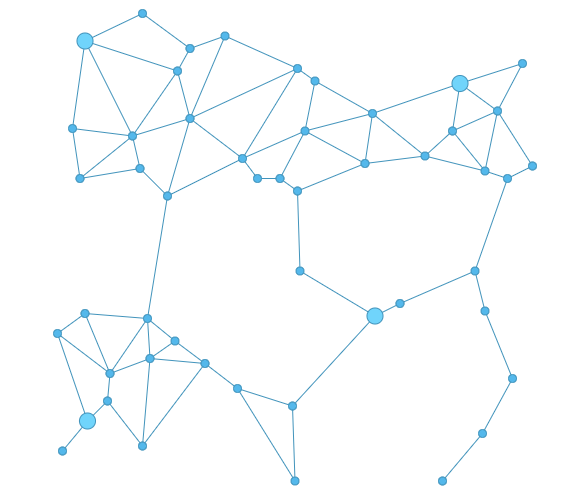
\includegraphics[width=0.5\textwidth]{images/map.png}\\
\end{figure}
\\
We were notified by the client of the capacity and the cost of production of each supplier, in MJ and \(\$/MJ\) respectively, as seen in the table below.
\renewcommand\baselinestretch{1.5}
\begin{table}[h]
    \centering
    \color{black}
    \begin{tabular}{|c:c:c:c:c|}
        \hline
        \textbf{Supplier Node} & \textbf{2} & \textbf{33} & \textbf{35} & \textbf{41} \\
        \hline
        \textbf{Capacity} (MJ)	& 462 & 955 &	957 & 704 \\ \hdashline
        \textbf{Cost} (\$/MJ) & 78	& 71 &	86 & 69\\
        \hline
    \end{tabular}
    \caption{Supplier Information}
    \label{tab:supinfo}
\end{table}
\renewcommand\baselinestretch{1}
\noindent
\\
It was also given that there is an additional charge associated with moving the gas of \$0.01 per MJ of gas per km of pipeline used. \\
\\
The remaining data was presented in two csv files, the first including the locations of the supplier and demand nodes, using X and Y coordinates, and the second file explaining which nodes connect on the network (a table representation of the network graph presented above). \\
\\
The goal of the project was to provide an optimal cost for meeting the current daily demand to the nodes from the suppliers, by minimising the total cost of production and distribution.\\
\\
After applying a Linear Programming (LP) model in Gurobi (via Python), it was found that the minimised optimal cost of supplying the gas would be \$172,468 (communication 1). \\
\\
\newpage
\noindent
The table below summarises the amount of gas produced by each supplier:
\renewcommand\baselinestretch{1.5}
\begin{table}[h]
    \centering
    \color{black}
    \begin{tabular}{|c:c|}
        \hline
        \textbf{Supplier Node} & \textbf{Gas Produced} (MJ)\\
        \hline
        2 & 462 \\ \hdashline
        33 & 955\\ \hdashline
        35 & 214 \\ \hdashline
        41 & 704\\ 
        \hline
    \end{tabular}
    \caption{Supplier Production}
    \label{tab:gasgenc1}
\end{table}
\renewcommand\baselinestretch{1}

\noindent
It is interesting to note that suppliers 2, 33 and 41 are producing to their maximum capacity, while supplier node 35 is not producing to its maximum capacity. Intuitively, this shows the cost of producing the gas further away (at a cheaper rate) and transporting it further outweighs the cost of producing the gas closer with a more expensive supplier.
\bigskip
\subsubsection{Communication 2}
In Communication 2, the clients informed us that there is an additional constraint regarding the maximum capacity of each pipeline. They specified that each pipeline can only handle a maximum of \(M = 452\) MJ per day. It was requested that we update the model to suit this added constraint. \\
\\
Upon adding this constraint, it was found that the new optimized cost was \$172,508 (communication 2). It can be seen that this added constraint increased the daily cost of the supply by \$40.\\
\\
There were only 2 pipelines that exceeded this daily gas flow limit, the original and limited gas flows have been summarised in the following table:\\
\renewcommand\baselinestretch{1.5}
\begin{table}[h]
    \centering
    \color{black}
    \begin{tabular}{|c:c:c|}
        \hline
        \textbf{Pipeline} (To Node, From Node) & \textbf{Original Gas Flow} (MJ) & \textbf{Limited Gas Flow} (MJ)\\
        \hline
        (22, 43) & 511 & 347\\ \hdashline
        (41, 22) & 616 & 452\\ 
        \hline
    \end{tabular}
    \caption{Original vs Limited Gas Flow}
    \label{tab:gasflow}
\end{table}
\renewcommand\baselinestretch{1}
\\
As can be seen from the table, the gas flow was limited at 452 MJ as required.
\newpage
\bigskip
\subsubsection{Communication 3}
In Communication 3 the client asked us to produce a new optimal cost over a 14 day period, in which the demand at each node varied daily. To do this we needed to update the model to account for the fortnightly period, as well as the fluctuating daily demand at each node, while ensuring that the total cost was given rather than a per day cost. \\
\\
After the new model was produced, the new optimized solution found that the fortnightly optimal cost would be \$2,460,782 (communication 3). \\
\\
Observe that this price is approximately 14 times the price of communication 2 - as we are now providing a cost for producing the gas over a two-week (14-day) period.\\
\\
The table below summarizes the new daily gas production for each supplier: 
\renewcommand\baselinestretch{1.5}
\begin{table}[h]
    \centering
    \color{black}
    \begin{tabular}{|c:c:c:c:c|}
        \hline
        \textbf{Day} & \textbf{Supplier Node 2} & \textbf{Supplier Node 35} & \textbf{Supplier Node 35} & \textbf{Supplier Node 41} \\ \hline
        Day 1 & 462 & 955 & 628 & 704 \\ \hdashline
        Day 2 & 462 & 955 & 721 & 704 \\ \hdashline
        Day 3 & 462 & 955 & 736 & 704 \\ \hdashline
        Day 4 & 462 & 955 & 715 & 704 \\ \hdashline
        Day 5 & 462 & 955 & 673 & 704 \\ \hdashline
        Day 6 & 0 & 709 & 0 &704 \\ \hdashline
        Day 7 & 0 & 264 & 0 & 704 \\ \hdashline
        Day 8 & 462 & 955 & 715 & 704 \\ \hdashline
        Day 9 & 462 & 955 & 646 & 704 \\ \hdashline
        Day 10 & 462 & 955 & 633 & 704 \\ \hdashline
        Day 11 & 462 & 955 & 639 & 704 \\ \hdashline
        Day 12 & 462 & 955 & 760 & 704 \\ \hdashline
        Day 13 & 0 & 647 & 0 &  704 \\ \hdashline
        Day 14 & 0 & 194 & 0 & 704 \\ \hline
    \end{tabular}
    \caption{Supplier Production per day for 14 days}
    \label{tab:supinfo2}
\end{table}
\renewcommand\baselinestretch{1}
\newpage
\bigskip
\subsubsection{Communication 4}
In Communication 4 the clients informed us that they wanted to balance out their market and spread out the amount of gas that each client could produce. They decided that there would be a limit of 10,227 MJ of natural gas per supplier over the 2-week period. \\
\\
After the model was improved to take into consideration this further constraint, it was found that the new fortnightly optimal cost would be \$2,467,681 (communication 4). This is a cost increase of \$6,899 for the fortnight. \\
\\
It is intuitive that there was such a large increase as the restricted supply resulted in the more expensive suppliers needing to produce a larger quantity of gas, as well as gas needing to travel further to reach each of the demand nodes.\\
\\
The table below summarizes the new daily production at each supply node:
\bigskip
\renewcommand\baselinestretch{1.5}
\begin{table}[h]
    \centering
    \color{black}
    \begin{tabular}{|c:c:c:c:c|}
        \hline
        \textbf{Day} & \textbf{Supplier Node 2} & \textbf{Supplier Node 35} & \textbf{Supplier Node 35} & \textbf{Supplier Node 41} \\ \hline
        Day 1 & 462 & 955 & 628 & 704 \\ \hdashline
        Day 2 & 462 & 955 & 721 & 704 \\ \hdashline
        Day 3 & 462 & 955 & 736 & 704 \\ \hdashline
        Day 4 & 462 & 955 & 715 & 704 \\ \hdashline
        Day 5 & 462 & 955 & 673 & 704 \\ \hdashline
        Day 6 & 431 & 278 & 0 &704 \\ \hdashline
        Day 7 & 181 & 83 & 0 & 704 \\ \hdashline
        Day 8 & 462 & 955 & 715 & 704 \\ \hdashline
        Day 9 & 462 & 955 & 646 & 704 \\ \hdashline
        Day 10 & 462 & 955 & 633 & 704 \\ \hdashline
        Day 11 & 462 & 955 & 639 & 704 \\ \hdashline
        Day 12 & 462 & 955 & 760 & 704 \\ \hdashline
        Day 13 & 412 & 235 & 0 &704 \\ \hdashline
        Day 14 & 113 & 81 & 0 & 704 \\ \hline
    \end{tabular}
    \caption{Limited Supplier Production per day for 14 days}
    \label{tab:supinfoc4}
\end{table}
\renewcommand\baselinestretch{1}


\newpage
\subsubsection{Communication 5}
The final communication from the client revealed that the pipelines can be considered as large storage containers that can be either over or under capacity based on the gas pressure within the pipes. This allows the clients to have a temporary deficit or surplus of gas within the pipes. However, any imbalance would result in a \$0.10/MJ cost to Pacific Paradise Gas, although it would allow for cheaper unused supply on lower demand days to be used on higher demand days. The company did set the restriction that the net imbalance must be 0 at the end of the fortnightly period.\\
\\
With this new information in mind, the model was able to be optimized to produce a new optimal cost of \underline{\textbf{\$2,460,287}} to meet the forecasted demand over the next two weeks. This is a decrease of \$7,394 from the previous solution, which is reasonable given that the cost of producing the gas would reduce, however, the same quantity of gas would need to be produced.\\
\\
Some checks were performed to determine the validity of the new optimized solution. In particular, the total gas produced was found to be \textbf{32,706 MJ} for both the models for communication 4 and communication 5. This shows that the same amount of gas is being produced in the revised model, just at a cheaper cost, which is the expected result as the forecasted demand has remained the same.\\
\\
It is worth noting a minor assumption that was made regarding the gas flow constraint from communication two when you informed us of the possibility for imbalance in communication five. Specifically, we have limited \textit{both} the gas flowing into and out of a pipe to be at most \(452 \hspace{0.1cm}\frac{MJ}{\text{day}}\). This instead of only constraining the inflow \textit{or} outflow of gas from each pipe.\\
\\
The summary table of the gas produced at each supplier node can be found below:

\renewcommand\baselinestretch{1.5}
\begin{table}[h]
    \centering
    \color{black}
    \begin{tabular}{|c:c:c:c:c|}
        \hline
        \textbf{Day} & \textbf{Supplier Node 2} & \textbf{Supplier Node 35} & \textbf{Supplier Node 35} & \textbf{Supplier Node 41} \\ \hline
        Day 1 & 462 & 894 & 564 & 704 \\ \hdashline
        Day 2 & 462 & 955 & 514 & 704 \\ \hdashline
        Day 3 & 462 & 955 & 503 & 704 \\ \hdashline
        Day 4 & 462 & 952 & 484 & 704 \\ \hdashline
        Day 5 & 462 & 912 & 502 & 704 \\ \hdashline
        Day 6 & 462 & 340 & 268 & 704 \\ \hdashline
        Day 7 & 462 & 193 & 175 & 704 \\ \hdashline
        Day 8 & 462 & 941 & 515 & 704 \\ \hdashline
        Day 9 & 462 & 899 & 542 & 704 \\ \hdashline
        Day 10 & 462 & 903 & 539 & 704 \\ \hdashline
        Day 11 & 462 & 886 & 529 & 704 \\ \hdashline
        Day 12 & 462 & 914 & 599 & 704 \\ \hdashline
        Day 13 & 462 & 298 & 263 & 704 \\ \hdashline
        Day 14 & 462 & 185 & 158 & 704 \\ \hline
    \end{tabular}
    \caption{Final Supplier Production per day for 14 days}
    \label{tab:gasgenb}
\end{table}
\renewcommand\baselinestretch{1}

\newpage
\bigskip
\subsection{Insight into solution}

\bigskip
%\subsubsection{Key Constraints of the Solution}
%\bigskip
%\subsubsection{Effects of Additional Requirements}
%\bigskip
%\subsubsection{Options on Costs}


\noindent
Using sensitivity analysis, we can investigate the impact of cost of limiting the maximum imbalance. To do so, the pipelines with a large imbalance on a particular day were then determined. Let \(I = 50\) MJ on a single day constitute a large imbalance. Using Gurobi, we can summarise the imbalances in these pipelines in the below table. There were a total of 12 distinct pipes that experienced an imbalance of this magnitude or greater across the two-week period.

\renewcommand\baselinestretch{1}
\begin{table}[h]
    \centering
    \color{black}
    \begin{tabular}{|c:c:c:c:c:c|}
        \hline
        \textbf{Day} \(t\) & \textbf{Pipe} \(p\) \textbf{(x, y)} & \(\delta_{p,t}\) & \textbf{Dual Value} & \(\delta_{p,t} - I\) & \textbf{Impact max imblnce} \(\$\) \\
        \hline
        1 & (34, 10) & 76.0 & 0.1 & 26.0 & 2.6 \\ \hdashline
        2 & (28, 31) & 88.0 & 0.1 & 38.0 & 3.8 \\ \hdashline
        2 & (12, 34) & 67.0 & 0.1 & 17.0 & 1.7 \\ \hdashline
        3 & (2, 48) & 54.0 & 0.1 & 4.0 & 0.4 \\ \hdashline
        3 & (28, 31) & 84.0 & 0.1 & 34.0 & 3.4 \\ \hdashline
        3 & (12, 34) & 69.0 & 0.1 & 19.0 & 1.9 \\ \hdashline
        4 & (22, 43) & 74.0 & 0.1 & 24.0 & 2.4 \\ \hdashline
        4 & (12, 34) & 55.0 & 0.1 & 5.0 & 0.5 \\ \hdashline
        5 & (28, 31) & 76.0 & 0.1 & 26.0 & 2.6 \\ \hdashline
        6 & (42, 18) & 193.0 & 0.1 & 143.0 & 14.3 \\ \hdashline
        6 & (28, 31) & 193.0 & 0.1 & 143.0 & 14.3 \\ \hdashline
        7 & (2, 48) & 93.0 & 0.1 & 43.0 & 4.3 \\ \hdashline
        7 & (29, 17) & 77.0 & 0.1 & 27.0 & 2.7 \\ \hdashline
        7 & (22, 36) & 131.0 & 0.1 & 81.0 & 8.1 \\ \hdashline
        7 & (12, 34) & 191.0 & 0.1 & 141.0 & 14.1 \\ \hdashline
        8 & (42, 18) & 95.0 & 0.1 & 45.0 & 4.5 \\ \hdashline
        8 & (22, 43) & 106.0 & 0.1 & 56.0 & 5.6 \\ \hdashline
        9 & (28, 31) & 59.0 & 0.1 & 9.0 & 0.9 \\ \hdashline
        10 & (18, 15) & 69.0 & 0.1 & 19.0 & 1.9 \\ \hdashline
        10 & (29, 17) & 77.0 & 0.1 & 27.0 & 2.7 \\ \hdashline
        11 & (28, 31) & 68.0 & 0.1 & 18.0 & 1.8 \\ \hdashline
        12 & (42, 18) & 64.0 & 0.1 & 14.0 & 1.4 \\ \hdashline
        13 & (28, 31) & 182.0 & 0.1 & 132.0 & 13.2 \\ \hdashline
        13 & (34, 10) & 169.0 & 0.1 & 119.0 & 11.9 \\ \hdashline
        14 & (18, 15) & 105.0 & 0.1 & 55.0 & 5.5 \\ \hdashline
        14 & (2, 12) & 118.0 & 0.1 & 68.0 & 6.8 \\ \hdashline
        14 & (2, 48) & 53.0 & 0.1 & 3.0 & 0.3 \\ \hdashline
        14 & (28, 46) & 94.0 & 0.1 & 44.0 & 4.4 \\ \hdashline
        14 & (5, 25) & 61.0 & 0.1 & 11.0 & 1.1 \\ \hdashline
        14 & (22, 43) & 180.0 & 0.1 & 130.0 & 13.0 \\
        \hline
    \end{tabular}
    \caption{Imbalance Constraint Sensitivity Analysis}
    \label{tab:constranals}
\end{table}
\renewcommand\baselinestretch{1.5}
\noindent
We can see there was indeed an imapact on cost of limiting the imbalance for any individual pipe ranging from less than \$1 to \$14.3 in pipes (42, 18) and (28, 31) on day 6.\\
\\
Interestingly, if we limited the model to have a maximum imbalance of 50 MJ per pipe per day, using the following constraint it was actually found that the new optimal cost was found to be the same at \(\$2,460,286.7\)! In words, we can describe this constraint as the difference in inflow and outflow of a pipe, denoted \(\delta_{p,t}\) is less than or equal to 50 for all pipes and for each day.\\
\\
This behaviour occurs because constraint sensitivity analysis only works when all other constraints are held constant, and so it wouldn't be correct to sum up all the cost savings.\\
\\
If one were to limit the imbalance down to 30 MJ per day per pipe, then we would see an increase in the total cost, but it seems when the imbalance can be at most 50 MJ, there are other pipes that can balance the imbalances with no impact on cost. Therefore, it can be concluded that would not be much of an impact on the cost by limiting this daily imbalance. 

\newpage
\subsection{Conclusion}
This network problem is constrained by the number of generators and their locations, the pipelines as well as the capacity and the cost of gas production. If Pacific Paradise Gas was able to reduce the cost of production at the supplier nodes, this could decrease their total cost of production and distribution. Or otherwise if they could increase their production capacity at the cheaper nodes, their production costs could be reduced. Alternatively, the construction of more pipelines between nodes would also allow for better balancing of gas through the pipes, and may even decrease the distance gas has to travel to reach it's destination. Finally, it could be worthwhile to build a new supplier node on the network that is strategically placed in order to reduce the distance between supplier nodes and demand nodes.



\bigskip
\color{black}
\end{document}